\documentclass[12pt]{article}

\usepackage{graphicx}
\usepackage{geometry}
\usepackage{multicol}
\usepackage{amsmath}

\geometry{
    top=20mm,
    bottom=20mm,
    right=20mm,
    left=20mm
}

\title{WMATH1010 Problem Set 3}
\author{Ben Crause || Aayush Bajaj}


\begin{document}
\maketitle{}

\section*{Question 1}
\[
    2\ln(x+2) + \frac{3}{2} \ln(x^2 + 6x + 13) + \frac{1}{2} \arctan(\frac{x}{2} + \frac{3}{2}) + C
\]

\section*{Question 2}

\subsection*{a)}
\[V = \frac{9 \pi}{10} u^3\]

\begin{center}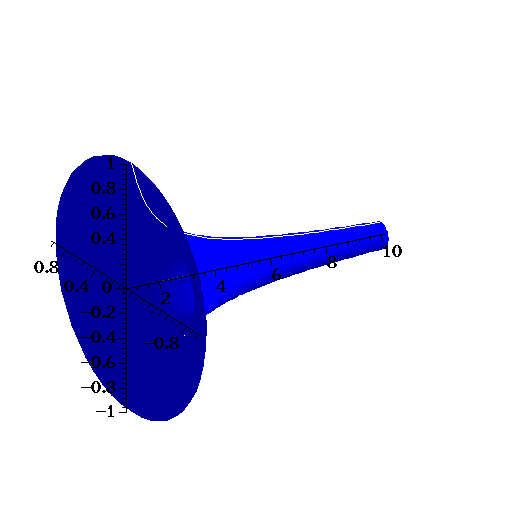
\includegraphics[width=0.5\textwidth, trim={2cm 1cm 2cm 3cm},clip]{plots/q2a.png}\end{center}
    %  trim={<left> <lower> <right> <upper>}

\newpage
\subsection*{b)}
\[
    V = \frac{\pi^2}{2}u^3    
\]
\begin{center}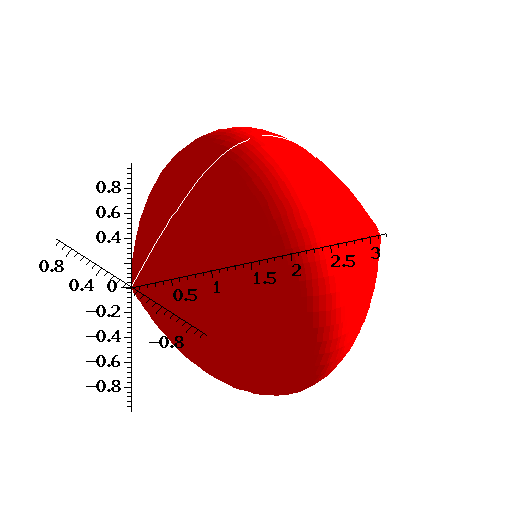
\includegraphics[width=0.5\textwidth, trim={2cm 1cm 2cm 3cm},clip]{plots/q2b.png}\end{center}

\subsection*{c)}
\[
    V = \frac{7533 \pi}{5} u^3
\]
\begin{center}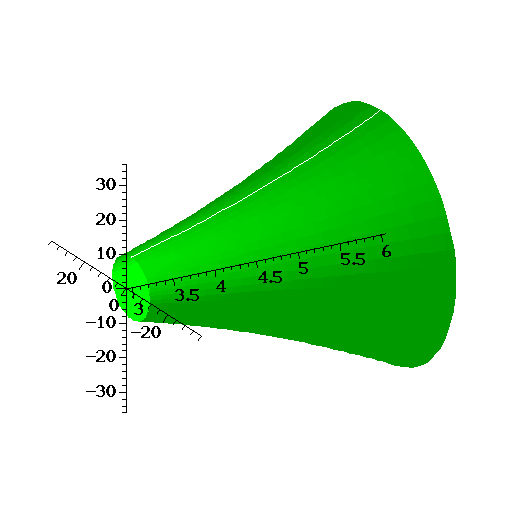
\includegraphics[width=0.5\textwidth, trim={2cm 1cm 2cm 3cm},clip]{plots/q2c.png}\end{center}

\newpage
\section*{Question 3}
\begin{align*}
    y_{\text{max}} &= 77.60 m \\
    t_{\text{total}} &= 7.96 s \\
    v &= 39 - 9.8t \\
    y &= 39t -4.9t^2
\end{align*}

\begin{multicols}{2}
    \includegraphics[width=0.5\textwidth]{plots/q3v.png}
    \includegraphics[width=0.5\textwidth]{plots/q3y.png}
\end{multicols}

\section*{Question 4}
\begin{align*}
    \text{A Bernoulli differential equation is of the form: }\\
    y' + p(x)y &= q(x)y^n\\
    \text{Hence:}\\
    p(x) &= x^5\\
    q(x) &= x^{12}\\
    n &= 0\\
\end{align*}
\begin{center}\includegraphics[width=0.9\textwidth]{ss.png}\end{center}

\end{document}
